\section{Routingprotokolle}

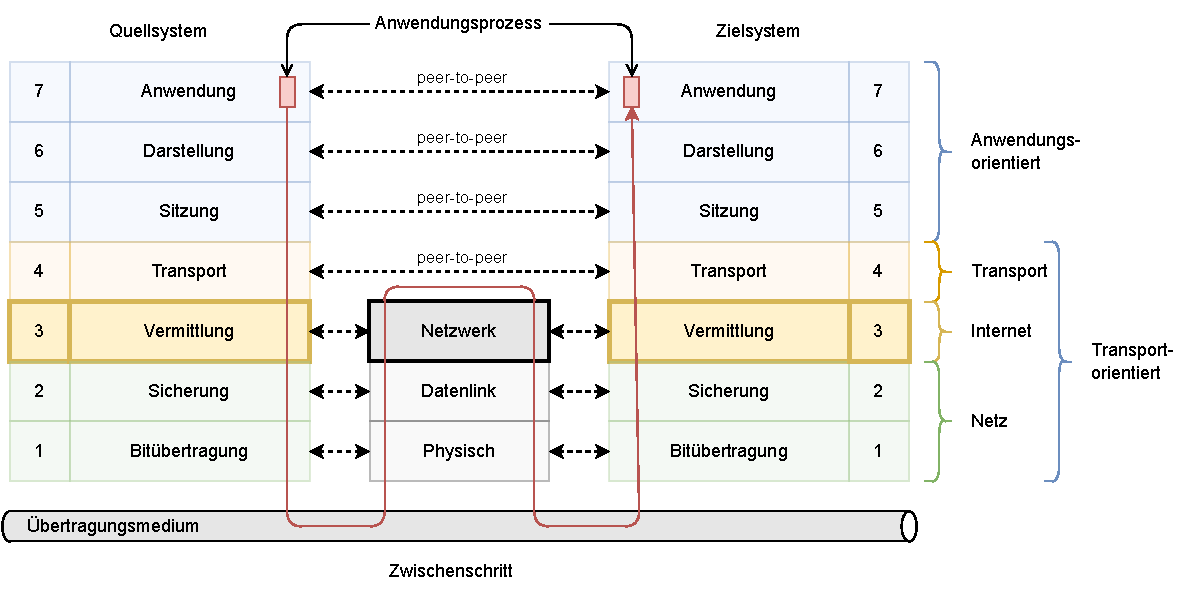
\includegraphics[width=\textwidth]{includes/figures/defi_iso_osi_network.pdf}

\begin{defi}{Routing}
    Das \emph{Weiterleiten (Routing)} erfüllt die wichtige Aufgabe, einzelne Teilstrecken des Kommunikationsnetzes so zu verbinden, dass eine Ende-zu-Ende-Kommunikation zwischen den angeschlossenen Teilnehmenden möglich wird.

    Das Routing kann in zwei Teilprozesse zerlegt werden:
    \begin{itemize}
        \item Das eigentliche Routing (die Control-Plane) ist verantwortlich für Wegewahl, mit der die Ende-zu-Ende-Kommunikation erreicht wird.
        \item Das Weiterleiten (Forwarding) der Pakete (die Data-Plane) gemäß den Vorgaben der Control-Plane.
    \end{itemize}

    Die Forwarding-Entscheidung wird für jedes Paket durchgeführt, unabhängig von vorherigen Entscheidungen, auf Basis der Zieladresse.
\end{defi}

\begin{bonus}{Routing-Metrik}
    Eine \emph{Routing-Metrik} ist ein numerischer Wert, mit dessen Hilfe ein Routing-Algorithmus feststellen kann, ob eine Route im Vergleich zu einer anderen besser ist.

    Metriken können Informationen wie z. B. Bandbreite, Verzögerung, Hop Count, Pfadkosten, Last, MTU, Verlässlichkeit und Kommunikationskosten berücksichtigen.
    Falls z. B. die Distanz die ausschlaggebende Metrik bei der Bestimmung einer Route ist, wird im Falle mehrerer möglicher Routen diejenige mit dem kleinsten Wert (d. h. der niedrigsten Distanz) gewählt.

    Nicht immer lässt sich aber die beste Route anhand des kleinsten Werts bestimmen, da z. B. eine höhere Bandbreite durch einen höheren Metrik-Wert repräsentiert wird.

    In der Routing-Tabelle werden oft nur die bestmöglichen Routen gehalten, während Link-State- oder topologische Datenbanken, aus denen die Routing-Tabelle gewonnen wird, sämtliche Informationen beinhalten.
\end{bonus}

\begin{defi}{Routing-Algorithmen}
    \emph{Routing-Algorithmen} benutzen zwei grundlegende Verfahrensweisen:
    \begin{itemize}
        \item Distanzvektor-Protokolle
        \item Link-State-Routing-Protokolle
    \end{itemize}
\end{defi}

\begin{defi}{Distanzvektor-Protokoll}
    \enquote{Teile deinen Nachbarn mit, wie für dich die Welt aussieht}: \emph{Distanzvektor-Protokolle} sorgen dafür, dass sich die Router untereinander nur mitteilen, wie gut sie an verschiedene Zielknoten angebunden sind.

    Vorgehen:
    \begin{enumerate}
        \item Jeder Router schickt regelmäßig seinen Nachbarn einen Distanzvektor, der die Kosten zu allen anderen Knoten im Netz enthält.
        \item Jeder Router aktualisiert daraufhin die eigene Liste mit den Kosten zu den anderen Knoten und wählt dabei den Weg mit den geringsten Kosten.
    \end{enumerate}

    Durch Auswahl des für ein bestimmtes Ziel optimalen Nachbarn wird die Lösung des Kürzeste-Wege-Problems somit auf mehrere Router verteilt.

    Ein Beispiel ist der \emph{Bellman-Ford-Algorithmus}.

    Vorteile:
    \begin{itemize}
        \item leicht zu implementieren
        \item einfache Berechnung
        \item neue, bessere Routen werden im Netz schnell propagiert
    \end{itemize}

    Nachteile:
    \begin{itemize}
        \item Ausfall von Routen bzw. Routern führt zum \emph{Count-to-Infinity-Problem}
    \end{itemize}
\end{defi}

\begin{defi}{Link-State-Routing-Protokoll}
    \enquote{Teile der Welt mit, wer deine Nachbarn sind}: \emph{Link-State-Routing-Protokolle} sorgen dafür, dass nach einiger Zeit jeder Router die vollständige Topologie des Netzwerks kennt und sich die kürzesten Wege darin selbst ausrechnen kann.

    Vorgehen:
    \begin{enumerate}
        \item Nachbarn und deren Netzadressen ermitteln
        \item Kosten zu jedem Nachbarn festlegen
        \item Paket zusammenstellen, in dem alles steht was bisher gelernt wurde
        \item Paket an alle anderen Router senden und von allen anderen Routern derartige Pakete empfangen
        \item kürzesten Pfad zu allen Routern berechnen
    \end{enumerate}

    Dadurch, dass die gesamte Topologie in jedem Router abgebildet ist, kann der Dijkstra-Algorithmus angewandt werden.

    Vorteile:
    \begin{itemize}
        \item optimale Lösung kann berechnet werden
        \item gute Performance bei Änderungen des Netzwerkes
    \end{itemize}

    Nachteile:
    \begin{itemize}
        \item höherer Rechenaufwand im Router
        \item höhere Komplexität bei der Versendung der Link-State-Pakete an alle anderen Router und deren Analyse
        \item höhere Netzlast
    \end{itemize}
\end{defi}

% \begin{example}{Link-State-Paket}
%     TODO
% \end{example}

\begin{algo}{Wiederholung Dijkstra-Algorithmus}
    Gegeben: Graph $G = (V, E)$, dessen Bewertungsfunktion die Eigenschaften hat:
    \begin{itemize}
        \item Jede Kante von $v_i$ nach $v_j$ hat nicht-negative Kosten: $C(i, j) \geq 0$
        \item Falls keine Kante zwischen $v_i$ und $v_j$: $C(i, j) = \infty$
        \item Diagonalelemente: $C(i, i) = 0$
    \end{itemize}

    Menge $S$: die Knoten, deren günstigste Wegekosten von der vorgegebenen Quelle (Startknoten) bereits bekannt sind.

    \begin{enumerate}
        \item Initialisierung: $S = \{ \text{Startknoten} \}$
        \item Beginnend mit Quelle alle ausgehenden Kanten betrachten (analog Breitensuche). Nachfolgerknoten $v$ mit günstigster Kante zu $S$ hinzunehmen.
        \item Jetzt: Berechnen, ob die Knoten in $V \setminus S$ günstiger über $v$ als Zwischenweg erreichbar sind, als ohne Umweg über $v$.
        \item Danach: Denjenigen Knoten $v'$ zu $S$ hinzunehmen, der nun am günstigsten zu erreichen ist. Bei zwei gleich günstigen Knoten wird ein beliebiger davon ausgewählt.
        \item Ab Schritt 3 wiederholen, bis alle Knoten in $S$ sind.
    \end{enumerate}

    Zeitkomplexität (bei Speicherung des Graphen mit Adjazenzmatrix): $\bigo(\abs{V}^2)$
\end{algo}

\begin{example}{Dijkstra-Algorithmus}
    \begin{center}
        \begin{tikzpicture}[->]
            \node[draw, circle] (A) {$A$};
            \node[draw, circle, below right=of A] (D) {$D$};
            \node[draw, circle, right=of D] (E) {$E$};
            \node[draw, circle, above right=of E] (B) {$B$};
            \node[draw, circle, below right=of B] (H) {$H$};
            \node[draw, circle, below left=of H] (G) {$G$};
            \node[draw, circle, below left=of A] (F) {$F$};
            \node[draw, circle, below right=of F] (C) {$C$};

            \path (A) edge node[weight, below left] {4} (D);
            \path (A) edge node[weight, above right] {2} (E);
            \path (A) edge node[weight, above right] {12} (B);
            \path (A) edge node[weight, above left] {30} (F);
            \path (E) edge node[weight, above] {1} (D);
            \path (E) edge node[weight, below right] {8} (C);
            \path (E) edge node[weight, above left] {8} (B);
            \path (C) edge node[weight, above right] {3} (F);
            \path (C) edge node[weight, above right] {3} (F);
            \path (C) edge node[weight, above] {12} (G);
            \path (G) edge node[weight, right] {4} (B);
            \path (G) edge node[weight, below right] {5} (H);
            \path (H) edge node[weight, above right] {2} (B);
        \end{tikzpicture}

        \vspace{1em}

        \begin{tabular}{|c|ccccccc|ccccccc|}
            \hline
            \multirow{2}{*}{$v_i$} & $d[2]$      & $d[3]$      & $d[4]$     & $d[5]$     & $d[6]$      & $d[7]$      & $d[8]$      & $p[2]$ & $p[3]$ & $p[4]$ & $p[5]$ & $p[6]$ & $p[7]$ & $p[8]$ \\ \cline{2-15}
                                   & B           & C           & D          & E          & F           & G           & H           & B      & C      & D      & E      & F      & G      & H      \\
            \hline
            A                      & 12          &             & 4          & \textbf{2} & 30          &             &             & A      &        & A      & A      & A      &        &        \\
            E                      & 10          & 10          & \textbf{3} & \textbf{2} & 30          &             &             & E      & E      & E      & A      & A      &        &        \\
            D                      & \textbf{10} & 10          & \textbf{3} & \textbf{2} & 30          &             &             & E      & E      & E      & A      & A      &        &        \\
            B                      & \textbf{10} & \textbf{10} & \textbf{3} & \textbf{2} & 30          &             &             & E      & E      & E      & A      & A      &        &        \\
            C                      & \textbf{10} & \textbf{10} & \textbf{3} & \textbf{2} & \textbf{13} & 22          &             & E      & E      & E      & A      & C      & C      &        \\
            F                      & \textbf{10} & \textbf{10} & \textbf{3} & \textbf{2} & \textbf{13} & \textbf{22} &             & E      & E      & E      & A      & C      & C      &        \\
            G                      & \textbf{10} & \textbf{10} & \textbf{3} & \textbf{2} & \textbf{13} & \textbf{22} & \textbf{27} & E      & E      & E      & A      & C      & C      & G      \\
            H                      & \textbf{10} & \textbf{10} & \textbf{3} & \textbf{2} & \textbf{13} & \textbf{22} & \textbf{27} & E      & E      & E      & A      & C      & C      & G      \\
            \hline
        \end{tabular}
    \end{center}

    \vspace{1em}

    \url{https://youtu.be/4pBP2hbnGso} (Herleitung und Erklärung)
\end{example}


\begin{algo}{Wiederholung Bellman-Ford-Algorithmus}
    Gegeben: Graph $G = (V, E)$, dessen Bewertungsfunktion die Eigenschaften hat:
    \begin{itemize}
        \item Falls keine Kante zwischen $v_i$ und $v_j$: $C(i, j) = \infty$
        \item Diagonalelemente: $C(i, i) = 0$
    \end{itemize}

    \begin{enumerate}
        \item Initialisierung: Startknoten $s$, Distanz zu $V \setminus \{s\}$ auf $\infty$ setzen
        \item Für jede Kante $(i, j)$:
              \begin{itemize}
                  \item Falls Distanz zu $v_i$ bekannt:
                        \subitem Falls $d(v_i) + C(i, j) < d(v_j)$, setze $d(v_j)$ auf $d(v_i) + C(i, j)$
              \end{itemize}
    \end{enumerate}

    Zeitkomplexität: $\bigo(\abs{V} \cdot \abs{E})$
\end{algo}

\begin{example}{Bellman-Ford-Algorithmus}
    \begin{center}
        \begin{tikzpicture}[->,baseline,anchor=north]
            \node[draw, circle] (S) {$S$};
            \node[draw, circle, above right=of S] (A) {$A$};
            \node[draw, circle, right=of A] (B) {$B$};
            \node[draw, circle, below right=of S] (C) {$C$};
            \node[draw, circle, right=of C] (D) {$D$};

            \path (S) edge node[weight, above left] {2} (A);
            \path (S) edge node[weight, below left] {5} (C);
            \path (A) edge node[weight, above] {4} (B);
            \path (C) edge node[weight, above] {2} (D);
            \path (C) edge node[weight, left] {-4} (A);
            \path (D) edge node[weight, right] {8} (B);
            \path (B) edge[bend left=10] node[weight, below right] {1} (C);
            \path (C) edge[bend left=10] node[weight, above left] {6} (B);
        \end{tikzpicture}
        %
        \hspace{5em}
        %
        \begin{tabular}{|c||c|c|c|c|c|}
            \hline
              & S & A        & B        & C        & D        \\
            \hline
            0 & 0 & $\infty$ & $\infty$ & $\infty$ & $\infty$ \\
            1 & 0 & 2        & $\infty$ & 5        & $\infty$ \\
            2 & 0 & 1        & 6        & 5        & 7        \\
            3 & 0 & 1        & 5        & 5        & 7        \\
            4 & 0 & 1        & 5        & 5        & 7        \\
            \hline
        \end{tabular}

        Keine Änderungen nach Schritt 3 $\implies$ Fertig!
    \end{center}
\end{example}

\begin{bonus}{Lokales vs. globales Routing}
    Jeder Rechner braucht eine Routing-Tabelle:
    \begin{itemize}
        \item im Internet:
              \begin{itemize}
                  \item meist Link-State-Verfahren\footnote{z. B. Dijkstra} innerhalb autonomer Systeme (Backbones)
                  \item Distanzvektor-Verfahren\footnote{z. B. Bellman-Ford} zur Koppluing autonomer Systeme
              \end{itemize}
        \item in Firmen bzw. Stadtnetzen:
              \begin{itemize}
                  \item können State-Link- oder Distanzvektor-Verfahren nutzen
                  \item meist sinnvoller: statische Konfiguration
              \end{itemize}
    \end{itemize}
\end{bonus}